\section{Preprocessing}\label{s:preprocessing}

% Enumerated list
\begin{enumerate}
    \item Dropping non-relevant columns.
    \item Encoding the categorical target variable.
    \item Handling missing values using median imputation.
    \item Scaling numerical features to standardize the data.
    \item Combining all preprocessing steps using \texttt{ColumnTransformer}.
\end{enumerate}

\subsection{Data Encoding and Splitting}
The target variable, \texttt{SpType-ELS}, a categorical variable, was encoded using \texttt{LabelEncoder} to convert categorical values into a binary numerical format. This transformation was essential for compatibility with the machine learning algorithms employed:

% Code example
\begin{verbatim}
label_encoder = LabelEncoder()
y_encoded = label_encoder.fit_transform(y)
\end{verbatim}

% Simple Table
Table \ref{tab:classifiers} summarizes the classifiers used, mapping them to the techniques discussed in class where applicable.
\begin{table}[h!]
    \centering
    \begin{tabular}{lll}
    \hline
    \textbf{Technique}          & \textbf{Concrete Method / Python Function} & \textbf{Week} \\
    \hline
    Decision Tree               & \texttt{DecisionTreeClassifier()}           & Week 7        \\
    Logistic Regression         & \texttt{LogisticRegression()}               & new           \\
    Random Forest               & \texttt{RandomForestClassifier()}            & Week 11       \\
    K-Nearest Neighbors         & \texttt{KNeighborsClassifier()}              & 444           \\
    Support Vector Classifier   & \texttt{SVC()}                               & Week 10       \\
    Multi-layer Perceptron      & \texttt{MLPClassifier()}                     & Week 9        \\
    XGBoost Classifier          & \texttt{XGBClassifier()}                     & new           \\
    Bagging Classifier          & \texttt{BaggingClassifier()}                 & Week 11       \\
    AdaBoost Classifier         & \texttt{AdaBoostClassifier()}                & Week 11       \\
    Gradient Boosting Classifier & \texttt{GradientBoostingClassifier()}        & new           \\
    \hline
    \end{tabular}
    \caption{Mapping of classifiers to discussed techniques in class}
    \label{tab:classifiers}
\end{table}


\subsection{Evaluation Workflow}
The best model and corresponding parameters were determined as follows: Two distinct settings were utilized, corresponding to two independent script executions, with one using 50\% and the other using 100\% of the available training data. The complete pipeline was then run for four different subsets of the data. Each pipeline employed \texttt{GridSearch} to identify the optimal parameters for ten different models. The parameter grid is shown in Table~\ref{tab:hyperparameters}: In total, 124 configurations, an in-depth distribution is depicted in Figure~\ref{fig:grid_search_analysis}, were evaluated using stratified 5-fold cross-validation. For each subset of features, the pipeline identified the best parameters based on model accuracy. The best model was then proposed and evaluated against the test data, with this final evaluation including multiple metrics.


% Complex table
% LaTeX command to adjust row height in tables
\renewcommand{\arraystretch}{1.5} % Adjust this value to increase/decrease row height

% Long table listing
\begin{longtable}[c]{c>{\raggedleft\arraybackslash}p{8cm}}
    \hline
    \textbf{Classifier} & \textbf{Parameter Grid} \\
    \hline
    \endfirsthead
    %
    \multicolumn{2}{c}%
    {{\bfseries Table \thetable\ continued from previous page}} \\
    \hline
    \textbf{Classifier} & \textbf{Parameter Grid} \\
    \hline
    \endhead
    %
    \hline
    \endfoot
    %
    \hline
    \hline
    %\multicolumn{2}{|c|}{End of Table} \\
    %\hline
    \endlastfoot
    %
    Decision Tree Classifier & \begin{tabular}[c]{@{}c@{}} max\_depth: [None, 10, 20, 30],\\ min\_samples\_split: [2, 10, 20],\\ min\_samples\_leaf: [1, 5, 10] \end{tabular} \\
    \hline
    Logistic Regression Classifier & \begin{tabular}[c]{@{}c@{}} C: [0.1, 1.0, 10],\\ solver: [liblinear, lbfgs] \end{tabular} \\
    \hline
    Random Forest Classifier & \begin{tabular}[c]{@{}c@{}} n\_estimators: [200, 300],\\ max\_features: [sqrt, log2] \end{tabular} \\
    \hline
    KNN (K-Nearest Neighbors) & \begin{tabular}[c]{@{}c@{}} n\_neighbors: [1, 3, 5],\\ weights: [uniform, distance] \end{tabular} \\
    \hline
    SVC (Support Vector Classifier) & \begin{tabular}[c]{@{}c@{}} C: [1, 2],\\ kernel: [rbf, sigmoid] \end{tabular} \\
    \hline
    MLPC (Multi-layer Perceptron Classifier) & \begin{tabular}[c]{@{}c@{}} hidden\_layer\_sizes: [(50,), (100,), (50, 50)],\\ activation: [tanh, relu],\\ learning\_rate\_init: [0.01, 0.1] \end{tabular} \\
    \hline
    XGBC (XGBoost Classifier) & \begin{tabular}[c]{@{}c@{}} n\_estimators: [100, 300],\\ max\_depth: [1, 2],\\ learning\_rate: [0.1, 0.3],\\ subsample: [0.7, 1],\\ colsample\_bytree: [0.7, 1] \end{tabular} \\
    \hline
    Bagging Classifier & \begin{tabular}[c]{@{}c@{}} n\_estimators: [10, 50, 100],\\ max\_samples: [0.5, 1.0],\\ max\_features: [0.5, 1.0] \end{tabular} \\
    \hline
    AdaBoost Classifier & \begin{tabular}[c]{@{}c@{}} n\_estimators: [50, 100],\\ learning\_rate: [0.01, 0.1, 1] \end{tabular} \\
    \hline
    Gradient Boosting Classifier & \begin{tabular}[c]{@{}c@{}} n\_estimators: [10, 100],\\ learning\_rate: [0.1, 0.3],\\ max\_depth: [3, 5] \end{tabular} \\
    \caption{Hyperparameters for each model to be tuned during \texttt{GridSearch}}
    \label{tab:hyperparameters}
\end{longtable}

% Figure with 2 subfigures with corresponding captions and one overall caption
\begin{figure}[H]
    \centering
    \begin{subfigure}[b]{0.45\linewidth}
        \centering
        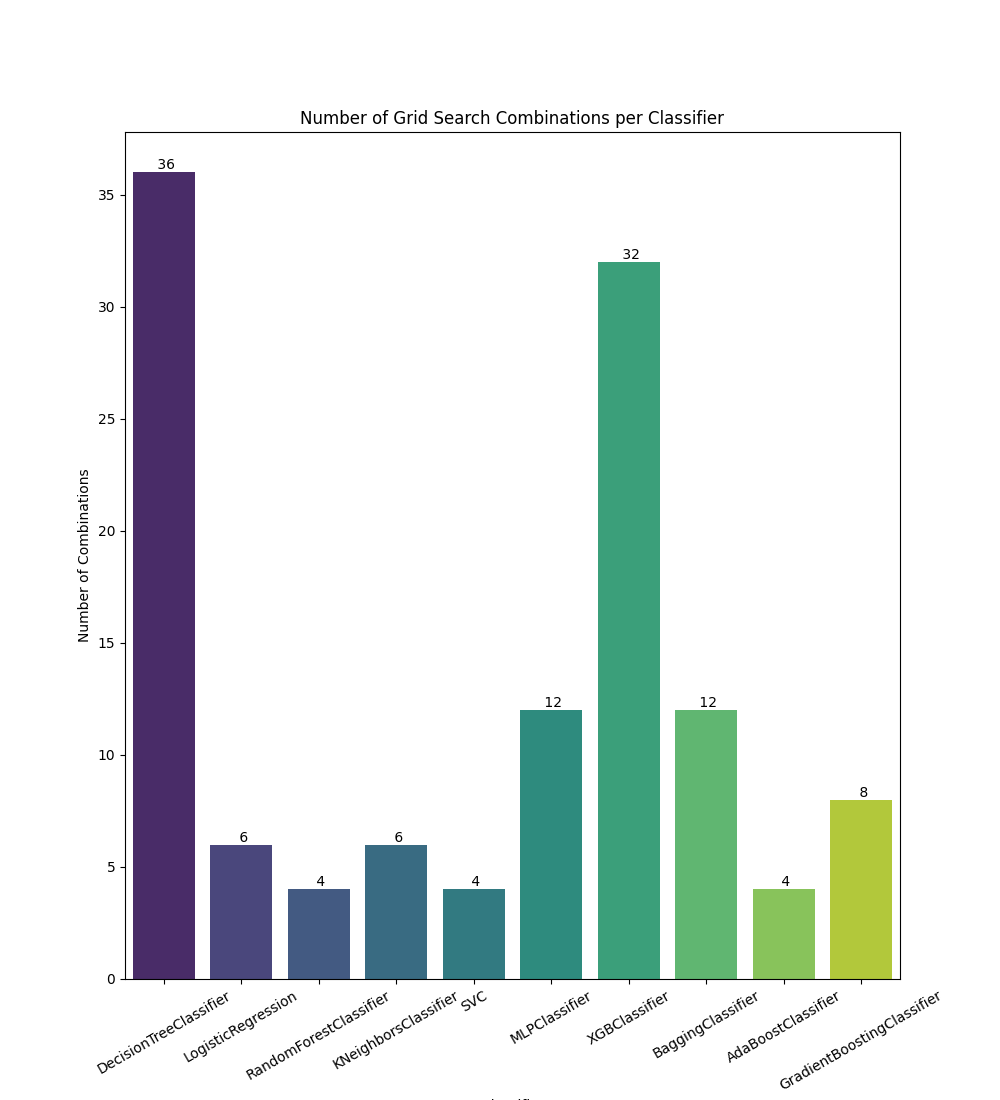
\includegraphics[width=\linewidth]{assets/images/methodology/grid_search_combinations_per_classifier.png}
        \caption{Number of \texttt{GridSearch} Combinations per Classifier (124 in total)}
        \label{fig:grid_search_combinations_per_classifier}
    \end{subfigure}
    \hfill
    \begin{subfigure}[b]{0.45\linewidth}
        \centering
        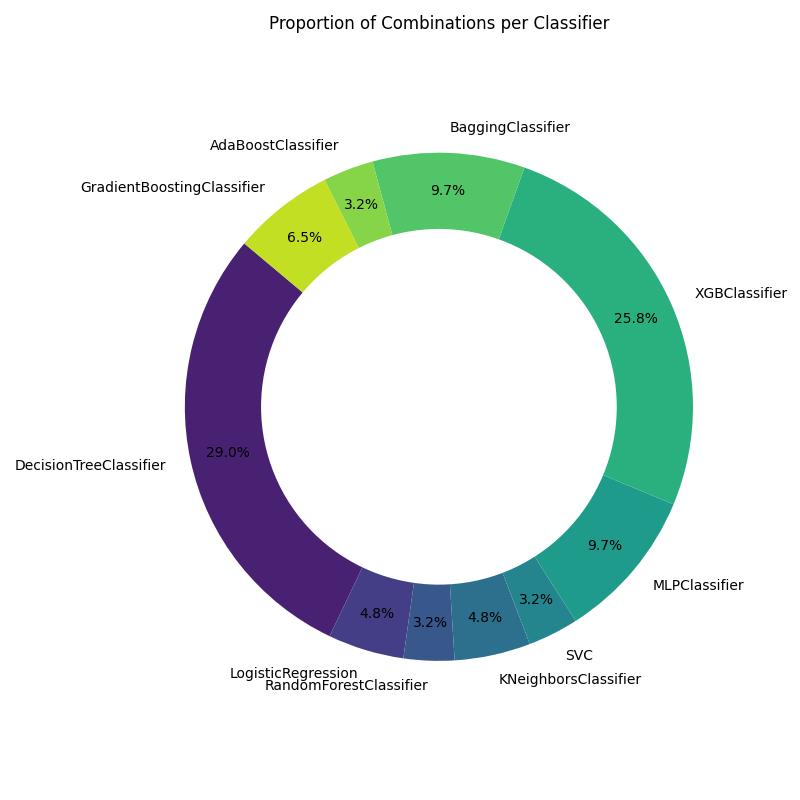
\includegraphics[width=\linewidth]{assets/images/methodology/grid_search_donat.png}
        \caption{Proportion of Combinations per Classifier}
        \label{fig:grid_search_donut}
    \end{subfigure}
    \caption{Analysis of \texttt{GridSearch} Combinations: The left plot shows the number of grid search combinations for each classifier, while the right plot illustrates the proportion of these combinations relative to the total combinations across all classifiers.}
    \label{fig:grid_search_analysis}
\end{figure}

% Full-width figure with one caption
\begin{figure}[H]
    \centering
    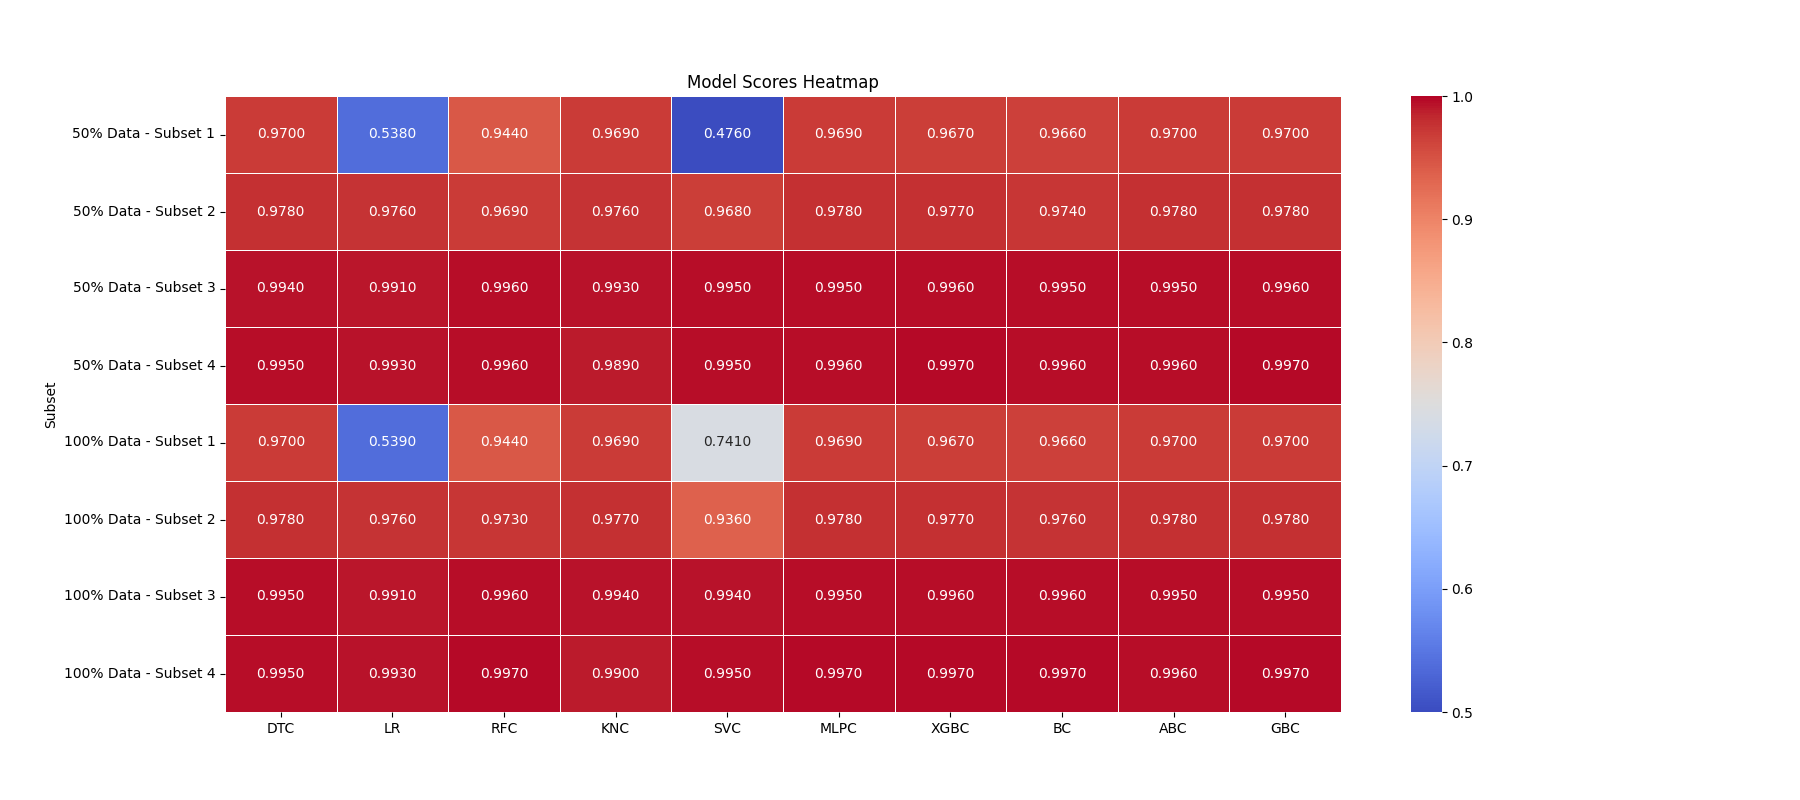
\includegraphics[trim=0cm 0cm 5cm 0cm, clip, width=\linewidth]{assets/images/best_classifier/eval_heatmap.png}
    \caption{Heatmap visualizing the performance of various models with optimal parameters across two different training data sizes (50\% and 100\%) and multiple feature sets. The scores are displayed with increased precision to highlight the subtle differences in model performance. This visualization aids in identifying the most effective models and configurations.}
    \label{fig:eval_heatmap}
\end{figure}
